%%%%%%%%%%%%%%%%%%%%%%%%%%%%%%%%%%%%%%%%%%%%%%%%%%%%%%%%%%%%%%%%%%%%%%%%%%%%%%%%
%% Plantilla de memoria en LaTeX para la EIF - Universidad Rey Juan Carlos
%%
%% Por Gregorio Robles <grex arroba gsyc.urjc.es>
%%     Grupo de Sistemas y Comunicaciones
%%     Escuela de Ingeniería de Fuenlabrada
%%     Universidad Rey Juan Carlos
%% (muchas ideas tomadas de Internet, colegas del GSyC, antiguos alumnos...
%%  etc. Muchas gracias a todos)
%%
%% La última versión de esta plantilla está siempre disponible en:
%%     https://github.com/gregoriorobles/plantilla-memoria
%%
%% Para obtener PDF, ejecuta en la shell:
%%   make
%% (las imágenes deben ir en PNG o JPG)

%%%%%%%%%%%%%%%%%%%%%%%%%%%%%%%%%%%%%%%%%%%%%%%%%%%%%%%%%%%%%%%%%%%%%%%%%%%%%%%%

\documentclass[a4paper, 12pt]{book}
%\usepackage[T1]{fontenc}

\usepackage[a4paper, left=2.5cm, right=2.5cm, top=3cm, bottom=3cm]{geometry}
\usepackage{times}
\usepackage[utf8]{inputenc}
\usepackage[spanish]{babel} % Comenta esta línea si tu memoria es en inglés
\usepackage{url}
%\usepackage[dvipdfm]{graphicx}
\usepackage{graphicx}
\usepackage{float}  %% H para posicionar figuras
\usepackage[nottoc, notlot, notlof, notindex]{tocbibind} %% Opciones de índice
\usepackage{latexsym}  %% Logo LaTeX

\title{Memoria del Proyecto}
\author{Paula Sepúlveda Membrilla}

\renewcommand{\baselinestretch}{1.5}  %% Interlineado

\begin{document}

\renewcommand{\refname}{Bibliografía}  %% Renombrando
\renewcommand{\appendixname}{Apéndice}


%%%%%%%%%%%%%%%%%%%%%%%%%%%%%%%%%%%%%%%%%%%%%%%%%%%%%%%%%%%%%%%%%%%%%%%%%%%%%%%%
% PORTADA

\begin{titlepage}
\begin{center}
\includegraphics[scale=0.6]{img/URJ_logo_Color_POS.png}

\vspace{1.75cm}

\LARGE
ESCUELA DE INGENIERÍA DE FUENLABRADA
\vspace{1cm}

\LARGE
GRADO EN INGENIERIA EN SISTEMAS AUDIOVISUALES Y MULTIMEDIA

\vspace{1cm}
\LARGE
\textbf{TRABAJO FIN DE GRADO}

\vspace{2cm}

\Large
TÍTULO DEL TRABAJO EN MAYÚSCULAS

\vspace{2cm}

\large
Autor : Paula Sepúlveda Membrilla \\
Tutor : Gregorio Robles Martínez\\
\vspace{1cm}

\large
Curso académico 2023/2024

\end{center}
\end{titlepage}

\newpage
\mbox{}
\thispagestyle{empty} % para que no se numere esta pagina



%%%%%%%%%%%%%%%%%%%%%%%%%%%%%%%%%%%%%%%%%%%%%%%%%%%%%%%%%%%%%%%%%%%%%%%%%%%%%%%%
%%%% Para firmar
\clearpage
\pagenumbering{gobble}
\chapter*{}

\vspace{-4cm}
\begin{center}
\LARGE
\textbf{Trabajo Fin de Grado}

\vspace{1cm}
\large
Título del Trabajo con Letras Capitales para Sustantivos y Adjetivos

\vspace{1cm}
\large
\textbf{Autor :} Paula Sepúlveda Membrilla \\
\textbf{Tutor :} Gregorio Robles Martínez
\end{center}

\vspace{1cm}
La defensa del presente Proyecto Fin de Carrera se realizó el día \qquad$\;\,$ de \qquad\qquad\qquad\qquad \newline de 202X, siendo calificada por el siguiente tribunal:


\vspace{0.5cm}
\textbf{Presidente:}

\vspace{1.2cm}
\textbf{Secretario:}

\vspace{1.2cm}
\textbf{Vocal:}


\vspace{1.2cm}
y habiendo obtenido la siguiente calificación:

\vspace{1cm}
\textbf{Calificación:}


\vspace{1cm}
\begin{flushright}
Fuenlabrada, a \qquad$\;\,$ de \qquad\qquad\qquad\qquad de 202X
\end{flushright}

%%%%%%%%%%%%%%%%%%%%%%%%%%%%%%%%%%%%%%%%%%%%%%%%%%%%%%%%%%%%%%%%%%%%%%%%%%%%%%%%
%%%% Dedicatoria

\chapter*{}
\pagenumbering{Roman} % para comenzar la numeracion de paginas en numeros romanos
\begin{flushright}
\textit{Dedicado a \\
mi familia / mi abuelo / mi abuela}
\end{flushright}

%%%%%%%%%%%%%%%%%%%%%%%%%%%%%%%%%%%%%%%%%%%%%%%%%%%%%%%%%%%%%%%%%%%%%%%%%%%%%%%%
%%%% Agradecimientos

\chapter*{Agradecimientos}
%\addcontentsline{toc}{chapter}{Agradecimientos} % si queremos que aparezca en el índice
\markboth{AGRADECIMIENTOS}{AGRADECIMIENTOS} % encabezado 

Aquí vienen los agradecimientos\ldots Aunque está bien acordarse de la pareja, no hay que olvidarse de dar las gracias a tu madre, que aunque a veces no lo parezca disfrutará tanto de tus logros como tú\ldots 
Además, la pareja quizás no sea para siempre, pero tu madre sí.

%%%%%%%%%%%%%%%%%%%%%%%%%%%%%%%%%%%%%%%%%%%%%%%%%%%%%%%%%%%%%%%%%%%%%%%%%%%%%%%%
%%%% Resumen

\chapter*{Resumen}
%\addcontentsline{toc}{chapter}{Resumen} % si queremos que aparezca en el índice
\markboth{RESUMEN}{RESUMEN} % encabezado

Aquí viene un resumen del proyecto.
Ha de constar de tres o cuatro párrafos, donde se presente de manera clara y concisa de qué va el proyecto. 
Han de quedar respondidas las siguientes preguntas:

\begin{itemize}
  \item ¿De qué va este proyecto? ¿Cuál es su objetivo principal?
  \item ¿Cómo se ha realizado? ¿Qué tecnologías están involucradas?
  \item ¿En qué contexto se ha realizado el proyecto? ¿Es un proyecto dentro de un marco general?
\end{itemize}

Lo mejor es escribir el resumen al final.

%%%%%%%%%%%%%%%%%%%%%%%%%%%%%%%%%%%%%%%%%%%%%%%%%%%%%%%%%%%%%%%%%%%%%%%%%%%%%%%%
%%%% Resumen en inglés

\chapter*{Summary}
%\addcontentsline{toc}{chapter}{Summary} % si queremos que aparezca en el índice
\markboth{SUMMARY}{SUMMARY} % encabezado

Here comes a translation of the ``Resumen'' into English. 
Please, double check it for correct grammar and spelling.
As it is the translation of the ``Resumen'', which is supposed to be written at the end, this as well should be filled out just before submitting.


%%%%%%%%%%%%%%%%%%%%%%%%%%%%%%%%%%%%%%%%%%%%%%%%%%%%%%%%%%%%%%%%%%%%%%%%%%%%%%%%
%%%%%%%%%%%%%%%%%%%%%%%%%%%%%%%%%%%%%%%%%%%%%%%%%%%%%%%%%%%%%%%%%%%%%%%%%%%%%%%%
% ÍNDICES %
%%%%%%%%%%%%%%%%%%%%%%%%%%%%%%%%%%%%%%%%%%%%%%%%%%%%%%%%%%%%%%%%%%%%%%%%%%%%%%%%

% Las buenas noticias es que los índices se generan automáticamente.
% Lo único que tienes que hacer es elegir cuáles quieren que se generen,
% y comentar/descomentar esa instrucción de LaTeX.

%%%% Índice de contenidos
\tableofcontents 
%%%% Índice de figuras
\cleardoublepage
%\addcontentsline{toc}{chapter}{Lista de figuras} % para que aparezca en el indice de contenidos
\listoffigures % indice de figuras
%%%% Índice de tablas
%\cleardoublepage
%\addcontentsline{toc}{chapter}{Lista de tablas} % para que aparezca en el indice de contenidos
%\listoftables % indice de tablas


%%%%%%%%%%%%%%%%%%%%%%%%%%%%%%%%%%%%%%%%%%%%%%%%%%%%%%%%%%%%%%%%%%%%%%%%%%%%%%%%
%%%%%%%%%%%%%%%%%%%%%%%%%%%%%%%%%%%%%%%%%%%%%%%%%%%%%%%%%%%%%%%%%%%%%%%%%%%%%%%%
% INTRODUCCIÓN %
%%%%%%%%%%%%%%%%%%%%%%%%%%%%%%%%%%%%%%%%%%%%%%%%%%%%%%%%%%%%%%%%%%%%%%%%%%%%%%%%

\cleardoublepage
\chapter{Introducción}
\label{chap:introducción}
\label{sec:intro} % etiqueta para poder referenciar luego en el texto con ~\ref{sec:intro}
\pagenumbering{arabic} % para empezar la numeración de página con números


En este capítulo se presenta la motivación que ha impulsado esta investigación,
proporcionando el contexto y las razones fundamentales para llevarla a cabo. A continuación, 
se define claramente el problema a resolver, especificando su alcance y relevancia, así como 
los objetivos que se desean alcanzar y las hipótesis planteadas al inicio del estudio.
\\Finalmente, se describe una visión general de cómo está organizado el documento y qué secciones lo componen.


\section{Motivación}
\label{sec:motivación}

La inspiración que me ha llevado a realizar este proyecto proviene de mi profesor y tutor, Gregorio Robles, quién me ha
motivado a adentrarme en el mundo del software libre (OSS, del inglés \textit{Open Source Software}).
\\El término software libre hace referencia al código diseñado de manera descentralizada y colaborativa, siendo
accesible para todo el público. Esto permite que cualquiera pueda utilizarlo, examinarlo, modificarlo y
redistribuirlo como considere conveniente.
\\La elección de código abierto nos aporta beneficios tales como un bajo coste, gran flexibilidad para
modificar el código fuente, así como un buen soporte proporcionado por parte de la comunidad.
Sin embargo, no existe una clara distinción entre el proceso de desarrollo y el de mantenimiento, lo cual resulta interesante
para la Ingeniería de Software al estudiar y explicar el funcionamiento de las interacciones que se llevan a cabo abiertamente.
\\Por lo tanto, la principal motivación de esta investigación es analizar el comportamiento de los proyectos de código abierto, los cuales se
desarrollan en una comunidad de usuarios que se comunican a través de distintas herramientas, teniendo como factor común Internet, lo que
permite guardar el registro de las actividades realizadas a lo largo del tiempo.
\\Además, este proyecto me ha brindado la oportunidad de adquirir conocimientos sobre minería de datos y desarrollar
habilidades para realizar un correcto análisis de los datos obtenidos.

\section{Definición del problema}
\label{sec:definición del problema}

El software libre permite a los desarrolladores realizar un completo análisis cuantitativo del
código y de todos los parámetros involucrados en su producción, debido a que están disponibles públicamente.
Al contar con datos de acceso público del desarrollo de software, permite llevar a cabo estudios estadísticos
para estudiar la evolución del software.
\\En todo este proceso, tiene gran importancia la utilización de un sistema de control de versiones, donde se permita
rastrear los cambios realizados en el pasado. De esta manera, podemos obtener un análisis de la estructura histórica
del código en base a sus distintas contribuciones, así como harían los arqueólogos estudiando una ciudad en base a sus
distintas construcciones.
Para software libre esto tiene vital importancia, ya que debido a la falta de diseño, el mantenimiento del código
es una actividad relevante para evitar posible código obsoleto de desarrolladores que ya no participan en el proyecto.


\\Aunque la Ingeniería de Software es una disciplina que se ha consolidado a través de los años, actualmente
existen muy pocos análisis empíricos sobre la arqueología del software. La falta de estudios junto con el atractivo hacia el
desarrollo comunitario del software libre, así como la importancia para la Ingeniería de Software de modelar con datos empíricos,
nos impulsa a llevar a cabo este proyecto.


\section{Objetivos e hipótesis}
\label{sec:objetivos}

Nuestra hipótesis es que, mediante un estudio empírico de las prácticas de desarrollo de software, la aplicación de minería de datos
al proyecto, el análisis de su evolución a lo largo del tiempo y la correlación de datos, se pueden determinar y aplicar métricas
que demuestren que la longevidad y el mantenimiento del código son heterogéneos y varían entre los diferentes componentes de varios proyectos.

\\Por lo que, el objetivo del proyecto consiste en estudiar la evolución y propiedades de varios proyectos de software libre a través del estudio
empírico, y en aplicar un análisis estadístico de su código fuente.
Se estudia el comportamiento de los proyectos FOSS\footnote{Free/Open Source Software}  más relevantes en GitHub, se identifican las fuentes de datos que ofrecen de manera pública y se presenta
una metodología para el análisis de los datos extraidos, que nos aportan datos interesantes a la investigación basados en la cantidad de colaboradores
o en los lenguajes de programación más utilizados.
De esta manera, podemos conocer mejor el fenómeno del software libre, el proceso de creación de software y cómo se puede aplicar en cualquier
otro entorno de desarrollo, se describe la mecánica de desarrollo de los movimientos de software libre.

\\Tenemos el objetivo de comprender el desarrollo de proyectos de software libre, así como la posibilidad de renovar la mecánica llevada a cabo mediante la
aplicación de los resultados obtenidos en esta investigación.

\section{Estructura de la memoria}
\label{sec:estructura}

A continuacion, describimos la estructura de la memoria, exponiendo el contenido de cada uno de los capítulos, proporcionando así
una guía organizada del trabajo de fin de grado para una mejor lectura y comprension de este.

\begin{itemize}
  
  \item \textbf{Capítulo~\ref{chap:introducción}: Introducción.}
  \\En este capítulo se describe la motivación que me ha llevado a realizar la investigación, así
  como el contexto, la definición del problema y las distintas hipótesis que se han desarrollado. Además, se ha ofrecido una breve descripción de la estructura del proyecto.

  \item \textbf{Capítulo~\ref{chap:objetivos}: Objetivos.}
  \\En este capítulo se describe el objetivo principal de la investigación, así como los objetivos específicos necesarios
  que van a guiar nuestro proyecto. Incluye una planificacion temporal de los objetivos mencionados. 
  
  \item \textbf{Capítulo~\ref{chap:estado}: Estado del arte.}
  \\En este capítulo se proporciona información detallada sobre el diseño, las características y los usos de cada
  una de las tecnologías y herramientas utilizadas en el proyecto.  
  
  \item \textbf{Capítulo~\ref{chap:diseño}: Diseño e implementación.}
  \\En este capítulo se detallan las fases que se han llevado a cabo para realizar el análisis de estudio. 
  Se describe la arquitectura general del proyecto, la mecánica de obtención y almacenamiento de los datos, y su posterior análisis empírico.

  \item \textbf{Capítulo~\ref{chap:resultados}: Resultados.}
  \\En este capítulo se describen los resultados obtenidos tras analizar los datos recopilados en el análisis, y se 
  realiza una justificación de dichos resultados.
 
  \item \textbf{Capítulo~\ref{chap:conclusiones}: Conclusiones.}
  \\En este capítulo se explican las conclusiones a las que se ha llegado, con su correspondiente justificación.
  Además, se mencionan los conocimientos adquiridos durante la duración de todo el grado universitario que se han aplicado en este proyecto, y los relacionados con el aprendizaje
  adquirido durante la realización de este estudio. Por último, se mencionan posibles mejoras que se pueden aplicar en el futuro.

\end{itemize}

%%%%%%%%%%%%%%%%%%%%%%%%%%%%%%%%%%%%%%%%%%%%%%%%%%%%%%%%%%%%%%%%%%%%%%%%%%%%%%%%
%%%%%%%%%%%%%%%%%%%%%%%%%%%%%%%%%%%%%%%%%%%%%%%%%%%%%%%%%%%%%%%%%%%%%%%%%%%%%%%%
% OBJETIVOS %
%%%%%%%%%%%%%%%%%%%%%%%%%%%%%%%%%%%%%%%%%%%%%%%%%%%%%%%%%%%%%%%%%%%%%%%%%%%%%%%%

\cleardoublepage % empezamos en página impar
\chapter{Objetivos} % título del capítulo (se muestra)
\label{chap:objetivos} % identificador del capítulo (no se muestra, es para poder referenciarlo)

En este capítulo, se definen los objetivos que guiarán la realización de este Trabajo de Fin de Grado (TFG).
Establecer objetivos claros y bien definidos es fundamental para asegurar una dirección precisa y coherente
a lo largo del desarrollo del proyecto.
\\Estos objetivos se dividen en dos categorías principales: el objetivo general,
que representa la meta global del trabajo, y los objetivos específicos, que son metas más concretas y detalladas necesarias
para alcanzar el objetivo general. 
\\Además, se presenta una planificación temporal que muestra la organización de las tareas a lo largo
del período de ejecución del proyecto, garantizando un avance ordenado y sistemático.

\section{Objetivo general} % título de sección (se muestra)
\label{sec:objetivo-general} % identificador de sección (no se muestra, es para poder referenciarla)

El objetivo general del proyecto es investigar en profundidad la evolución y las características de proyectos de software libre
alojados en la plataforma de GitHub mediante un estudio empírico detallado y la aplicación estadística de su código fuente. 
A través de este enfoque, se pretende obtener una comprensión íntegra de cómo el proyecto ha cambiado y se ha desarrollado a lo
largo del tiempo, identificando patrones, tendencias y características del código que puedan influir en su calidad, mantenibilidad y eficiencia.
\\Esta investigación no solo implica un análisis histórico, sino que también incluye la aplicacion de diversas métricas
para evaluar distintos aspectos del código fuente. 
Al combinar métodos empíricos con análisis estadísticos robustos, este proyecto busca proporcionar una visión detallada y objetiva
del comportamiento evolutivo del software.
\\Los resultados obtenidos nos ofrecen conclusiones y recomendaciones para la mejora continua del desarrollo del software libre,
contribuyendo al conocimiento en el campo de Ingeniería de Software que puede aplicarse en la toma de decisiones en proyectos futuros.

\section{Objetivos específicos}
\label{sec:objetivos-especificos}

Para lograr el objetivo general detallado en el proyecto se han establecido los siguientes objetivos específicos:
\begin{itemize}
  
  \item \textbf{Investigación.}
  \\Consiste en buscar y evaluar información sobre el contexto de trabajo, realizando una estimación de los
  costes de desarrollo software. Se piensa como desarrollar la programación de manera eficiente, y a su vez se realiza una selección de distintos
  repositorios de GitHub que resultan de especial interés para nuestra investigación.

  \item \textbf{Programación.}
  \\En esta fase del proyecto se desarrollan los scripts necesarios para extraer, almacenar y analizar los datos con
  el fin de conseguir los objetivos de esta investigación.
  
  \item \textbf{Recopilación de datos.}
  \\En esta etapa se recopilan y almacenan los datos más relevantes para el posterior estudio del comportamiento
  de los repositorios seleccionados.  
  
  \item \textbf{Análisis estadístico.}
  \\Tras la recopilación de los datos, se ajustan y configuran las métricas correspondientes para obtener
  distintas estadísticas sobre la evolución de los repositorios a lo largo del tiempo.

  \item \textbf{Representación gráfica.}
  \\Una vez que se ha realizado un análisis estadístico, se realiza un análisis empírico y se representan 
  de manera gráfica los resultados obtenidos.
 
  \item \textbf{Documentación.}
  \\En esta etapa se elaboran la documentación y los informes necesarios para la correcta entrega del Trabajo de Fin de Grado (TFG).

\end{itemize}


\section{Planificación temporal}
\label{sec:planificacion-temporal}

\begin{figure}
  \centering
  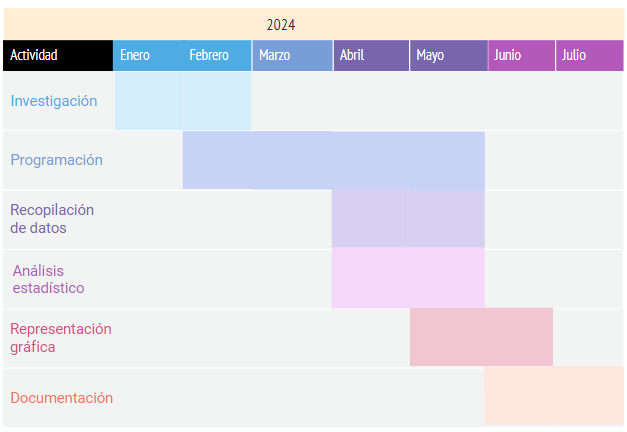
\includegraphics[width=14cm, keepaspectratio]{img/Diagrama_Gantt.png}
  \caption{Diagrama de Gantt}
  \label{fig:diagrama_gantt}
\end{figure}

El desarrollo de este proyecto abarca un período de siete meses, desde enero de 2024 hasta julio de 2024, con la realización de un trabajo diario que se lleva a cabo
de manera constante. En la figura~\ref{fig:diagrama_gantt} se observa el tiempo empleado en las diferentes fases del proyecto, donde se puede
observar que varias tareas se han solapado en algunos casos debido al avance en paralelo de distintas actividades.
\begin{itemize}
  
  \item \textbf{Enero 2024}
  \\En este mes comienzo el desarrollo de esta investigación, cuando mi tutor Gregorio Robles me sugirió la idea del proyecto.
  Comienzan las reuniones donde se definen los objetivos correspondientes, y empiezo a documentarme para obtener los conocimientos
  necesarios para la realización del proyecto.
  \\Recopilo información acerca de los proyectos de código abierto y posibles repositorios de especial interés que son alojados en la plataforma de GitHub.
  A su vez, estudio la información que se puede obtener de las líneas de código mediante el comando \textit{git blame}, y que análisis nos puede
  resultar de interés para estudiar la evolución de estos repositorios a lo largo de los años.

  \item \textbf{Febrero 2024}
  \\Durante este mes sigo realizando la tarea de investigación, pero además trabajo en paralelo con la tarea de programación. Comienzo a 
  desarrollar el código de programación basado en el comando \textit{git blame}, mediante el cual obtengo información interesante acerca de
  los cambios realizados en un archivo específico línea por línea. El comando \textit{git blame} nos proporciona información del autor de la línea de código, así como de la fecha del commit, del estado de
  esa línea y obviamente podemos ver también su contenido.
  
  \item \textbf{Marzo 2024}
  \\En este mes me centro exclusivamente en la programación del código, desarrollando los scripts \textit{init.py} y \textit{git-blameall.py}. Estos scripts
  analizan un repositorio y un archivo respectivamente, con el objetivo de analizar línea a línea cada uno de los archivos de un repositorio, y guardan los datos recogidos en un archivo JSON.
  \\Al principio, se trabaja en realizar el análisis para un único archivo y finalmente se logra conseguir analizar un repositorio concreto. Además, se estudia
  la opción de tener que analizar las distintas versiones de un archivo o unicamente la versión final, quedandonos con la segunda opción al ser mucho más eficiente y 
  conseguir obtener los datos que nos interesan.
  
  \item \textbf{Abril 2024}
  \\Este mes tiene una gran carga de trabajo, al realizar en paralelo tres actividades distintas. Por una parte, sigo avanzando con la programación, mejorando los scripts \textit{init.py} y \textit{git-blameall.py}
  de manera que los datos pasan de guardarse en un archivo JSON a guardarse en tres bases de datos relacionadas entre sí: \textit{repositories}, \textit{files} y \textit{code} respectivamente.
  Esto requiere de un estudio previo para obtener los conocimientos necesarios sobre la utilización de \textit{MySQL} y el concepto de bases de datos relacionales. El hecho de almacenar los datos en bases de datos
  relacionales nos permite un posterior análisis de los datos de manera mucho más eficiente.

  \item \textbf{Mayo 2024}
  \\Durante estas semanas la carga de trabajo sigue siendo muy alta, desarrollando cuatro actividades de manera paralela. Termino de desarrollar los archivos de programación, incluido entre ellos el script \textit{graphics.py}
  que tiene como finalidad poder obtener una representación gráfica de las métricas estudiadas. A su vez, termino de definir los índices y las métricas que se incluyen en este proyecto, para obtener estadísticas interesantes
  acerca de la evolución de cambios, número de autores o posible código obsoleto en un repositorio. Seguidamente, se recopilan los últimos datos de los repositorios elegidos para su análisis, todos ellos alojados en la plataforma
  de GitHub.

  \item \textbf{Junio 2024}
  \\En esta etapa se elaboran las gráficas definitivas, y mientras tanto se empieza a escribir la memoria de nuestro proyecto.

  \item \textbf{Julio 2024}
  \\En este último mes se termina de escribir la memoria y se realizan las correcciones oportunas por el tutor para poder realizar una correcta entrega del Trabajo de Fin de Grado (TFG).


\end{itemize}


%%%%%%%%%%%%%%%%%%%%%%%%%%%%%%%%%%%%%%%%%%%%%%%%%%%%%%%%%%%%%%%%%%%%%%%%%%%%%%%%
%%%%%%%%%%%%%%%%%%%%%%%%%%%%%%%%%%%%%%%%%%%%%%%%%%%%%%%%%%%%%%%%%%%%%%%%%%%%%%%%
% ESTADO DEL ARTE %
%%%%%%%%%%%%%%%%%%%%%%%%%%%%%%%%%%%%%%%%%%%%%%%%%%%%%%%%%%%%%%%%%%%%%%%%%%%%%%%%

\cleardoublepage
\chapter{Estado del arte}
\label{chap:estado}

En este capítulo, se presentan las herramientas y librerías usadas en el Trabajo Fin de Grado.
Esta exposicion nos da una visión de las tecnologías empleadas en el proyecto.

\section{Tecnologías y herramientas} 
\label{sec:seccion1}

\subsection{Python}
\label{subsec:estilo}

---
\subsection{GitHub}
\label{subsec:estilo}

\subsection{MySQL}
\label{subsec:estilo}

\subsection{LaTeX}
\label{subsec:estilo}

\section{Librerías} 
\label{sec:seccion1}

\subsection{pyodbc}
\label{subsec:estilo}

\subsection{subprocess}
\label{subsec:estilo}

\subsection{sys}
\label{subsec:estilo}

\subsection{matplotlib}
\label{subsec:estilo}

\begin{table}
 \begin{center}
  \begin{tabular}{ | l | c | r |} % tenemos tres colummnas, la primera alineada a la izquierda (l), la segunda al centro (c) y la tercera a la derecha (r). El | indica que entre las columnas habrá una línea separadora.
    \hline
    Uno & 2 & 3 \\ \hline % el hline nos da una línea vertical
    Cuatro & 5 & 6 \\ \hline
    Siete & 8 & 9 \\
    \hline
  \end{tabular}
  \caption{Ejemplo de tabla. Aquí viene una pequeña descripción (el \emph{caption}, el pie de tabla/figura) del contenido de la tabla. Si la tabla no es autoexplicativa, siempre viene bien aclararla aquí.}
  \label{tab:ejemplo}
 \end{center}
\end{table}

Hay un sitio en Internet donde puedes diseñar las tablas fácilmente y luego hacer un corta y pega del resultado en tu editor.
Puedes probarlo en \url{https://www.tablesgenerator.com/}.

Hemos hablado de cómo incluir figuras.
Pero no hemos dicho nada de tablas.
A mí me gustan las tablas.
Mucho.
Aquí un ejemplo de tabla, la Tabla~\ref{tab:ejemplo} (siento ser pesado, pero nota cómo he puesto la referencia).



%%%%%%%%%%%%%%%%%%%%%%%%%%%%%%%%%%%%%%%%%%%%%%%%%%%%%%%%%%%%%%%%%%%%%%%%%%%%%%%%
%%%%%%%%%%%%%%%%%%%%%%%%%%%%%%%%%%%%%%%%%%%%%%%%%%%%%%%%%%%%%%%%%%%%%%%%%%%%%%%%
% DISEÑO E IMPLEMENTACIÓN %
%%%%%%%%%%%%%%%%%%%%%%%%%%%%%%%%%%%%%%%%%%%%%%%%%%%%%%%%%%%%%%%%%%%%%%%%%%%%%%%%

\cleardoublepage
\chapter{Diseño e implementación}
\label{chap:diseño}
\label{sec:diseno}

Aquí viene todo lo que has hecho tú (tecnológicamente). 
Puedes entrar hasta el detalle. 
Es la parte más importante de la memoria, porque describe lo que has hecho tú.
Eso sí, normalmente aconsejo no poner código, sino diagramas.



\section{Arquitectura general} 
\label{sec:arquitectura}

Si tu proyecto es un software, siempre es bueno poner la arquitectura (que es cómo se estructura tu programa a ``vista de pájaro'').

\begin{figure}
  \centering
  \includegraphics[width=9cm, keepaspectratio]{img/arquitectura.png}
  \caption{Estructura del parser básico}
  \label{fig:arquitectura}
\end{figure}


Por ejemplo, puedes verlo en la figura~\ref{fig:arquitectura}.
\LaTeX \ pone las figuras donde mejor cuadran. 
Y eso quiere decir que quizás no lo haga donde lo hemos puesto\ldots 
Eso no es malo.
A veces queda un poco raro, pero es la filosofía de \LaTeX: tú al contenido, que yo me encargo de la maquetación.


 
Recuerda que toda figura que añadas a tu memoria debe ser explicada.
Sí, aunque te parezca evidente lo que se ve en la figura~\ref{fig:arquitectura}, la figura en sí solamente es un apoyo a tu texto.
Así que explica lo que se ve en la figura, haciendo referencia a la misma tal y como ves aquí.
Por ejemplo: En la figura~\ref{fig:arquitectura} se puede ver que la estructura del \emph{parser} básico, que consta de seis componentes diferentes: los datos se obtienen de la red, y según el tipo de dato, se pasará a un \emph{parser} específico y bla, bla, bla\ldots

Si utilizas una base de datos, no te olvides de incluir también un diagrama de entidad-relación.


%%%%%%%%%%%%%%%%%%%%%%%%%%%%%%%%%%%%%%%%%%%%%%%%%%%%%%%%%%%%%%%%%%%%%%%%%%%%%%%%
%%%%%%%%%%%%%%%%%%%%%%%%%%%%%%%%%%%%%%%%%%%%%%%%%%%%%%%%%%%%%%%%%%%%%%%%%%%%%%%%
% EXPERIMENTOS Y VALIDACIÓN %
%%%%%%%%%%%%%%%%%%%%%%%%%%%%%%%%%%%%%%%%%%%%%%%%%%%%%%%%%%%%%%%%%%%%%%%%%%%%%%%%

\cleardoublepage
\chapter{Experimentos y validación}
\label{chap:experimentos}

Este capítulo se introdujo como requisito en 2019. 
Describe los experimentos y casos de test que tuviste que implementar para validar tus resultados. 
Incluye también los resultados de validación que permiten afirmar que tus resultados son correctos. 


%%%%%%%%%%%%%%%%%%%%%%%%%%%%%%%%%%%%%%%%%%%%%%%%%%%%%%%%%%%%%%%%%%%%%%%%%%%%%%%%
%%%%%%%%%%%%%%%%%%%%%%%%%%%%%%%%%%%%%%%%%%%%%%%%%%%%%%%%%%%%%%%%%%%%%%%%%%%%%%%%
% RESULTADOS %
%%%%%%%%%%%%%%%%%%%%%%%%%%%%%%%%%%%%%%%%%%%%%%%%%%%%%%%%%%%%%%%%%%%%%%%%%%%%%%%%

\cleardoublepage
\chapter{Resultados}
\label{chap:resultados}

En este capítulo se incluyen los resultados de tu trabajo fin de grado.

Si es una herramienta de análisis lo que has realizado, aquí puedes poner ejemplos de haberla utilizado para que se vea su utilidad.


%%%%%%%%%%%%%%%%%%%%%%%%%%%%%%%%%%%%%%%%%%%%%%%%%%%%%%%%%%%%%%%%%%%%%%%%%%%%%%%%
%%%%%%%%%%%%%%%%%%%%%%%%%%%%%%%%%%%%%%%%%%%%%%%%%%%%%%%%%%%%%%%%%%%%%%%%%%%%%%%%
% CONCLUSIONES %
%%%%%%%%%%%%%%%%%%%%%%%%%%%%%%%%%%%%%%%%%%%%%%%%%%%%%%%%%%%%%%%%%%%%%%%%%%%%%%%%

\cleardoublepage
\chapter{Conclusiones}
\label{chap:conclusiones}


\section{Consecución de objetivos}
\label{sec:consecucion-objetivos}

Esta sección es la sección espejo de las dos primeras del capítulo de objetivos, donde se planteaba el objetivo general y se elaboraban los específicos.

Es aquí donde hay que debatir qué se ha conseguido y qué no. 
Cuando algo no se ha conseguido, se ha de justificar, en términos de qué problemas se han encontrado y qué medidas se han tomado para mitigar esos problemas.

Y si has llegado hasta aquí, siempre es bueno pasarle el corrector ortográfico, que las erratas quedan fatal en la memoria final.
Para eso, en Linux tenemos aspell, que se ejecuta de la siguiente manera desde la línea de \emph{shell}:

\begin{verbatim}
  aspell --lang=es_ES -c memoria.tex
\end{verbatim}

\section{Aplicación de lo aprendido}
\label{sec:aplicacion}

Aquí viene lo que has aprendido durante el Grado/Máster y que has aplicado en el TFG/TFM.
Una buena idea es poner las asignaturas más relacionadas y comentar en un párrafo los conocimientos y habilidades puestos en práctica.

\begin{enumerate}
  \item a
  \item b
\end{enumerate}


\section{Lecciones aprendidas}
\label{sec:lecciones_aprendidas}

Aquí viene lo que has aprendido en el Trabajo Fin de Grado/Máster.

\begin{enumerate}
  \item Aquí viene uno.
  \item Aquí viene otro.
\end{enumerate}


\section{Trabajos futuros}
\label{sec:trabajos_futuros}

Ningún proyecto ni software se termina, así que aquí vienen ideas y funcionalidades que estaría bien tener implementadas en el futuro.

Es un apartado que sirve para dar ideas de cara a futuros TFGs/TFMs.


%%%%%%%%%%%%%%%%%%%%%%%%%%%%%%%%%%%%%%%%%%%%%%%%%%%%%%%%%%%%%%%%%%%%%%%%%%%%%%%%
%%%%%%%%%%%%%%%%%%%%%%%%%%%%%%%%%%%%%%%%%%%%%%%%%%%%%%%%%%%%%%%%%%%%%%%%%%%%%%%%
% APÉNDICE(S) %
%%%%%%%%%%%%%%%%%%%%%%%%%%%%%%%%%%%%%%%%%%%%%%%%%%%%%%%%%%%%%%%%%%%%%%%%%%%%%%%%

\cleardoublepage
\appendix
\chapter{Manual de usuario}
\label{app:manual}

Esto es un apéndice.
Si has creado una aplicación, siempre viene bien tener un manual de usuario.
Pues ponlo aquí.

%%%%%%%%%%%%%%%%%%%%%%%%%%%%%%%%%%%%%%%%%%%%%%%%%%%%%%%%%%%%%%%%%%%%%%%%%%%%%%%%
%%%%%%%%%%%%%%%%%%%%%%%%%%%%%%%%%%%%%%%%%%%%%%%%%%%%%%%%%%%%%%%%%%%%%%%%%%%%%%%%
% BIBLIOGRAFIA %
%%%%%%%%%%%%%%%%%%%%%%%%%%%%%%%%%%%%%%%%%%%%%%%%%%%%%%%%%%%%%%%%%%%%%%%%%%%%%%%%

\cleardoublepage

% Las siguientes dos instrucciones es todo lo que necesitas
% para incluir las citas en la memoria
\bibliographystyle{abbrv}
\bibliography{memoria}  % memoria.bib es el nombre del fichero que contiene
% las referencias bibliográficas. Abre ese fichero y mira el formato que tiene,
% que se conoce como BibTeX. Hay muchos sitios que exportan referencias en
% formato BibTeX. Prueba a buscar en http://scholar.google.com por referencias
% y verás que lo puedes hacer de manera sencilla.
% Más información: 
% http://texblog.org/2014/04/22/using-google-scholar-to-download-bibtex-citations/

\end{document}
